\chapter{Determinarea diametrului la butuc}\label{chapter:butuc}

\section{Calculul diametrului la butuc}

Notații:
\begin{itemize}
    \item D $[m]$ - diametru
    \item R $[m]$ - rază
\end{itemize}

\

\noindent
Indici:
\begin{itemize}
    \item p - periferie
    \item b - butuc
    \item s - stagnare
    \item m - mijloc
\end{itemize}

\

Pentru a calcula diametrul la butuc $D_b$ folosim teoria dezvoltată la Timișoara de Susan-Resiga si exemplificată în \cite{susanhub}, care ne permite calculul teoretic al razei de stagnare fără a mai fi necesar un proces iterativ empiric pana la obținerea unei valori care elimina riscul desprinderilor de pe butuc. Astfel începem prin calculul parametrul (adimensional) de intensitate a rotației $\sigma$.

Conform ecuației fundamentale a turbomașinilor (ecuația lui Euler) avem viteza tangențială la periferie:

\begin{equation}
gH=UV_{up}, \text{ sau } gH=\frac{\pi n}{30} R_{p} V_{up} \Rightarrow V_{up}=\frac{30gH}{\pi n R_{p}}
\end{equation}

Viteza axiala medie (debitanta) prind conductă este:

\begin{equation}
V_{ad}=\frac{Q}{\pi R_{p}^2}
\end{equation}

În ambele ecuații, (2.1) și (2.2) raza conductei este practic raza de la periferie a turbinei. Ca rezultat, parametrul (adimensional) de intensitate a rotației este:

\begin{equation}
\sigma \equiv \frac{V_{up}}{V_{ad}} = 30 \frac{g H R_{p}}{n Q} = 7.4
\end{equation}

Pentru o rotație cu circulație constantă și o presiune totală constantă în conducta a fost derivata in lucrarea \cite{susanhub} o ecuație algebrică pentru $x$, dedusa cu parametrul $\sigma$:

\begin{equation}
\frac{\sigma^2}{x^2} - \frac{2}{(1-x^3)} = 0
\end{equation}

Din (2.4) putem calcula raza de stagnare $R_{s}$ folosind metoda dezvoltata de Lebedev \cite{lebedev1991formulae} de rezolvare a ecuațiilor polinomiale de gradul 3 și obținem o valoare pentru $x$.

\begin{equation}
x = 0.73
\end{equation}

În regiunea (necunoscută) stagnantă $R_{s}$, se indică raportul de raza de stagnare fata de raza la periferie, totul la pătrat, de unde putem obține raza de stagnare:

\begin{equation}
\text{Definim } x \equiv \bigg(\frac{R_{s}}{R_{p}}\bigg)^2 \Rightarrow R_{s} = \sqrt{x} R_{p} = 0.094\si{m}
\end{equation}

\begin{figure}[h!]
	\centering
	\includegraphics[scale=0.6]{figures/radius_stag-sigma.eps}
	\caption{Raportul dintre raza regiunii stagnante și raza țevii față de intensitatea rotației, pentru o rotație cu circulație constantă și o presiune totală constantă \cite{susanhub}}
	\label{Raportul dintre raza regiunii stagnante și raza țevii față de intensitatea rotației}
\end{figure}

În Figura 2.1 putem observa corelația dintre intensitatea rotației pe abscise și raportul dintre raza de stagnare și raza la periferie a turbinei pe ordonata.

\begin{figure}[h!]
	\centering
	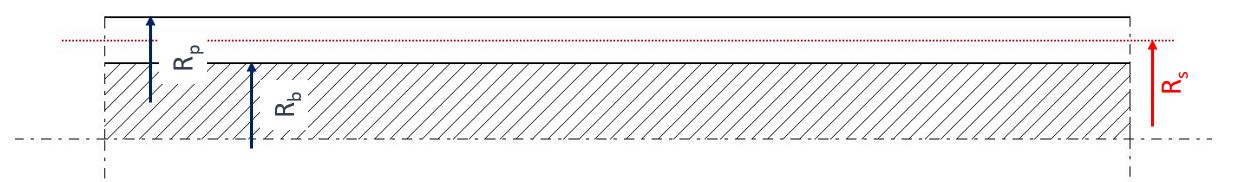
\includegraphics[scale=0.5]{figures/radii.jpg}
	\caption{Reprezentarea grafică a razelor din conducta în secțiune \cite{susanhub}}
	\label{Reprezentarea grafică a razelor din conducta în secțiune}
\end{figure}

După cum se poate observa în Figura 2.2, la o valoare a razei de butuc egala sau mai mare decât raza de stagnare, înlăturam riscurile conform teoriei enunțate inițial. Astfel se alege pentru raza la butuc aceeași valoare ca și a razei de stagnare și anume $0.094\si{m}$.

\begin{equation}
R_b \geq R_s = 0.094\si{m}
\end{equation}

\clearpage